\chapter{Edwards curves}
\label{cha:edwardsCurves}
In \cite{edwards07} Edwards gave a new normal form for elliptic curves. He showed that every elliptic curve over a field $\F$ of characteristic not 2, can be written as $x^2+y^2=c^2+c^2x^2y^2$ over a finite extension field of $\F$. In \cite{BL07} Bernstein and Lange generalized Edwards notion to $x^2+y^2=c^2(1+dx^2y^2)$ to allow more elliptic curves to be written in Edwards form without an extension of the underlying field. 

In this chapter $\F$ denotes a field with $\Char(\F)\neq 2$ if nothing else is stated. It is possible to define Edwards curves over binary fields (see \cite{binaryEdwards}) which in particular is interesting for implementing elliptic cryptography using Edwards curves on chips and smart cards. 

\section{Edwards curves}
\label{sec:EdwardC}
We now define Edwards cruves. Consider the curve 
\[	\overline{x}^2+\overline{y}^2=\overline{c}^2(1+\overline{d}\overline{x}^2\overline{y}^2),\quad \overline{c}\neq 0.
\]
This curve is isomorphic to 
\[
	x^2+y^2=1+dx^2y^2, \quad d=\overline{d}\overline{c}^4,
\]
which follows from the map $(\overline{x},\overline{y})\mapsto (\overline{c}x,\overline{c}y)$.
\begin{defn}\label{def:edwardsCurve}
Let $d\in\F\backslash\{0,1\}$. An Edwards curve over $\F$ is a curve on the from 
\begin{align}\label{rel:EC}
	x^2+y^2=1+dx^2y^2
\end{align}
with $d\in\F\backslash\{0,1\}$. We denote the Edwards curve by $E_{E,d}$. 
\end{defn}
Both Euler and Gauss has worked on the special case $d=-1$. In \cite{gaussWerke} Gauss presented addition formulas for that particular case; $(s,c)+(s',c')=\left(\frac{sc'+s'c}{1-ss'cc'},\frac{cc'-ss'}{1+ss'cc'}\right)$. With his choice of $s$ and $c$ he probably hinted to the connection with the addition laws for sine and cosine (look at the numerators and try to remember how the additions formulas for sine and cosine looks like). For more on this analogy see remark \ref{ex:clockGroup}.
\begin{rem}
The reason for not allowing $d=0$ or $d=1$ is the following. If $d=0$ then $x^2+y^2=1$ which is a genus 0 curve, not an elliptic curve (Generally an elliptic curve is a projective non singular genus 1 curve. This definition is equivalent with the one given in definition \ref{def:edwardsCurve} by the Riemann-Roch theorem). If $d=1$ then $0=1+x^2y^2-x^2-y^2=(y^2-1)(x^2-1)$ which again does not describe an elliptic curve. 
%Actually $x^2+y^2=1+dx^2y^2$ has two singularities at infinity $[1,0,0]$ and $[0,1,0]$ but these can be resolved by a ''blow up´´ technique describe in \cite{fulton1989algebraic} chapter 7.  
\end{rem}
\begin{figure}[htp]
\begin{minipage}[b]{0.5\linewidth}
\centering
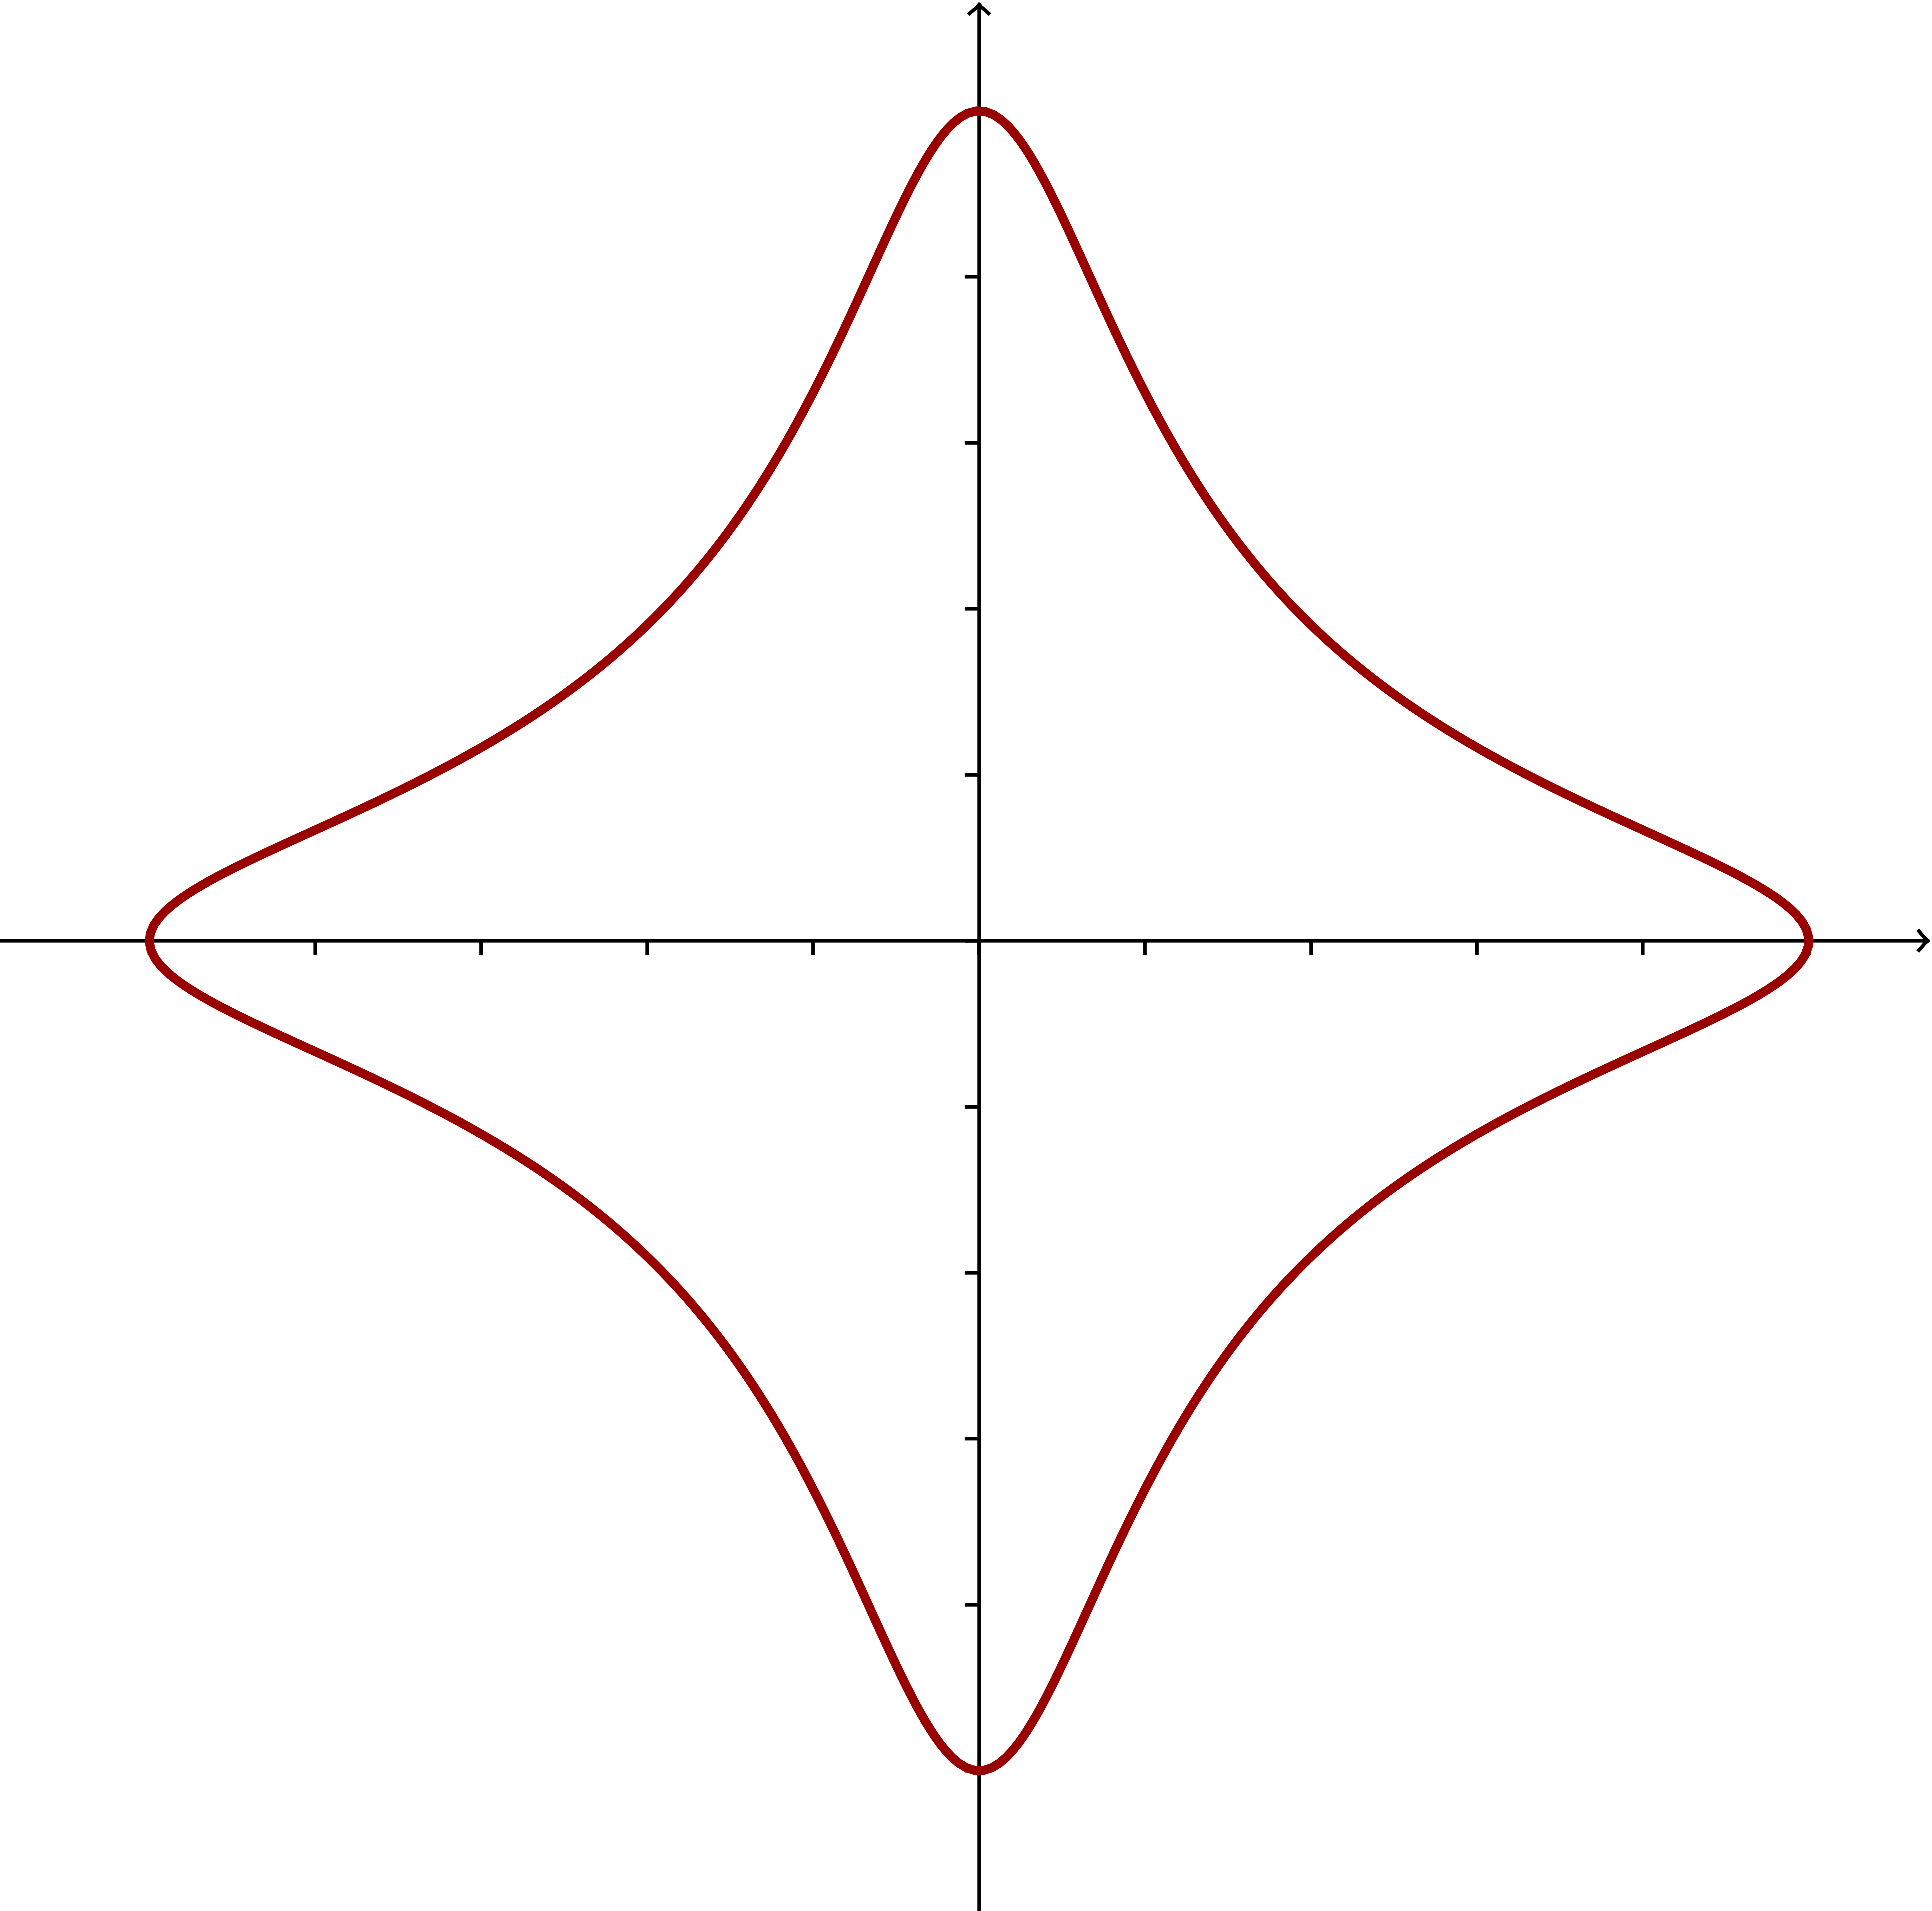
\includegraphics[scale=0.2]{edwards_curve_negative.png}
\caption{Edwards curve $E_{E,-30}$ over $\R$.}
\end{minipage}
\hspace{0.5cm}
\begin{minipage}[b]{0.5\linewidth}
\centering
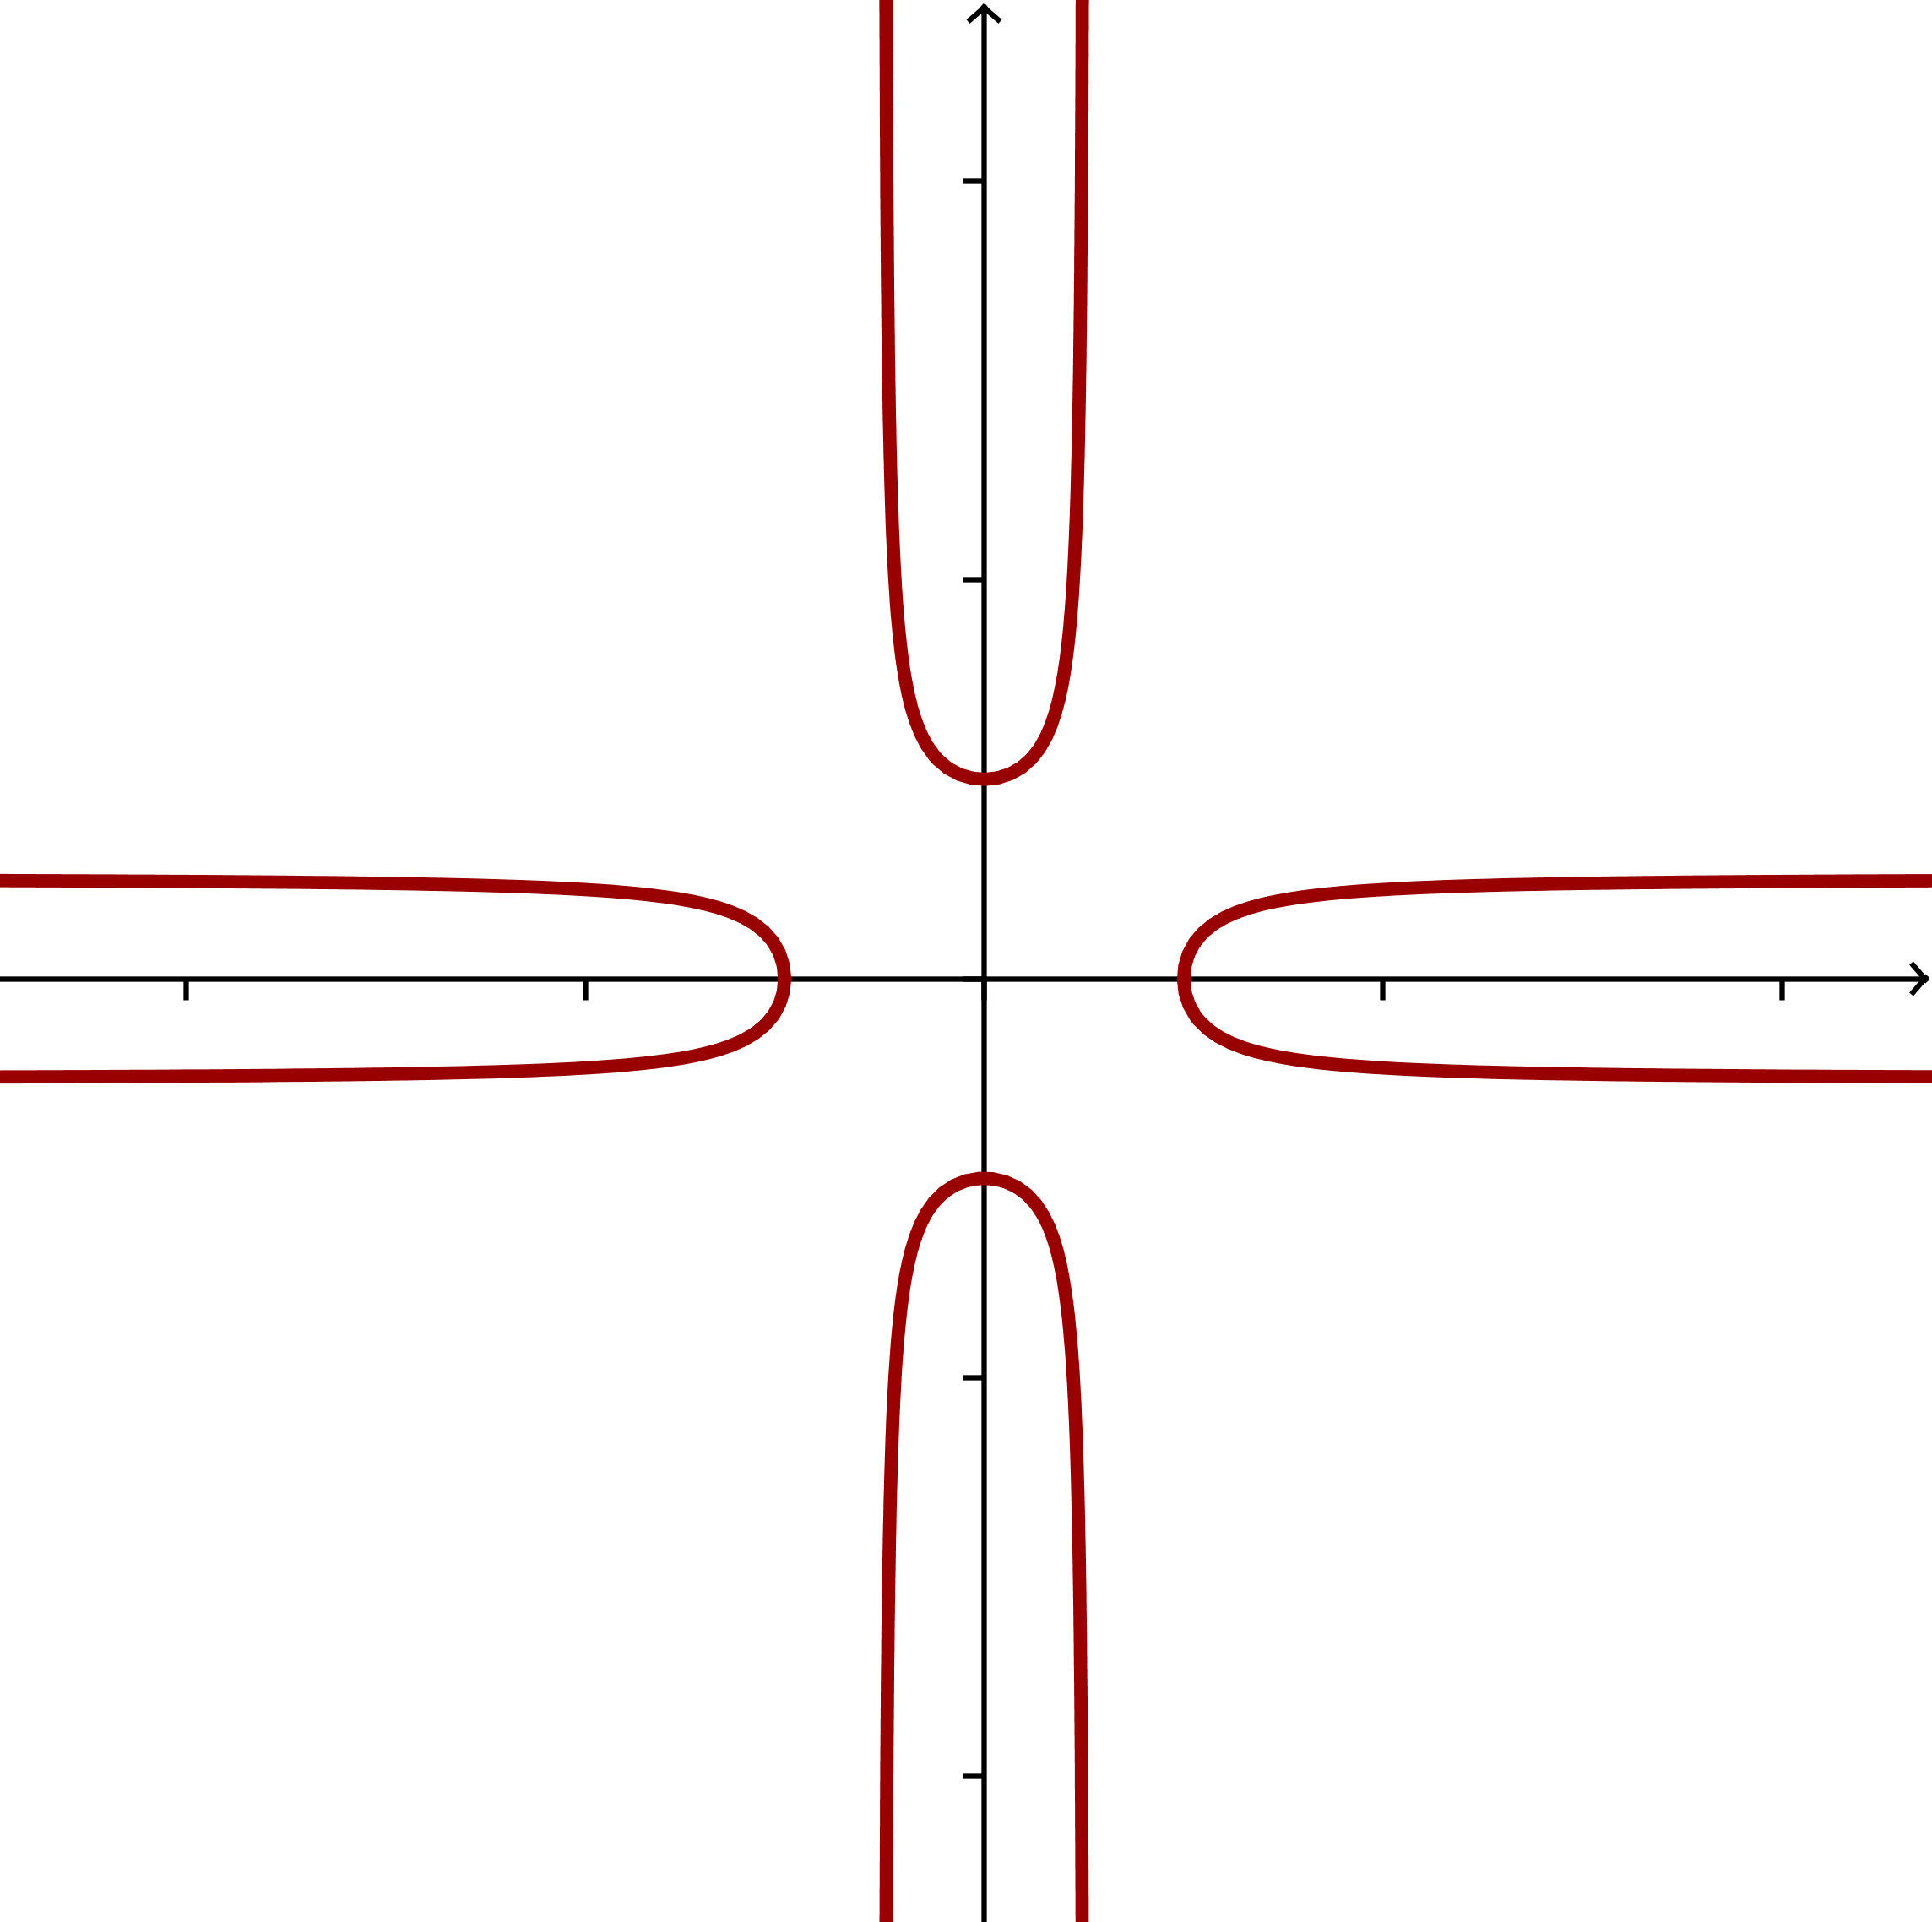
\includegraphics[scale=0.5]{edwards_curve_positive.png}
\caption{Edwards curve $E_{E,4}$ over $\R$.}
\end{minipage}
\end{figure}
\begin{figure}[h]
\begin{minipage}[b]{0.5\linewidth}
\centering
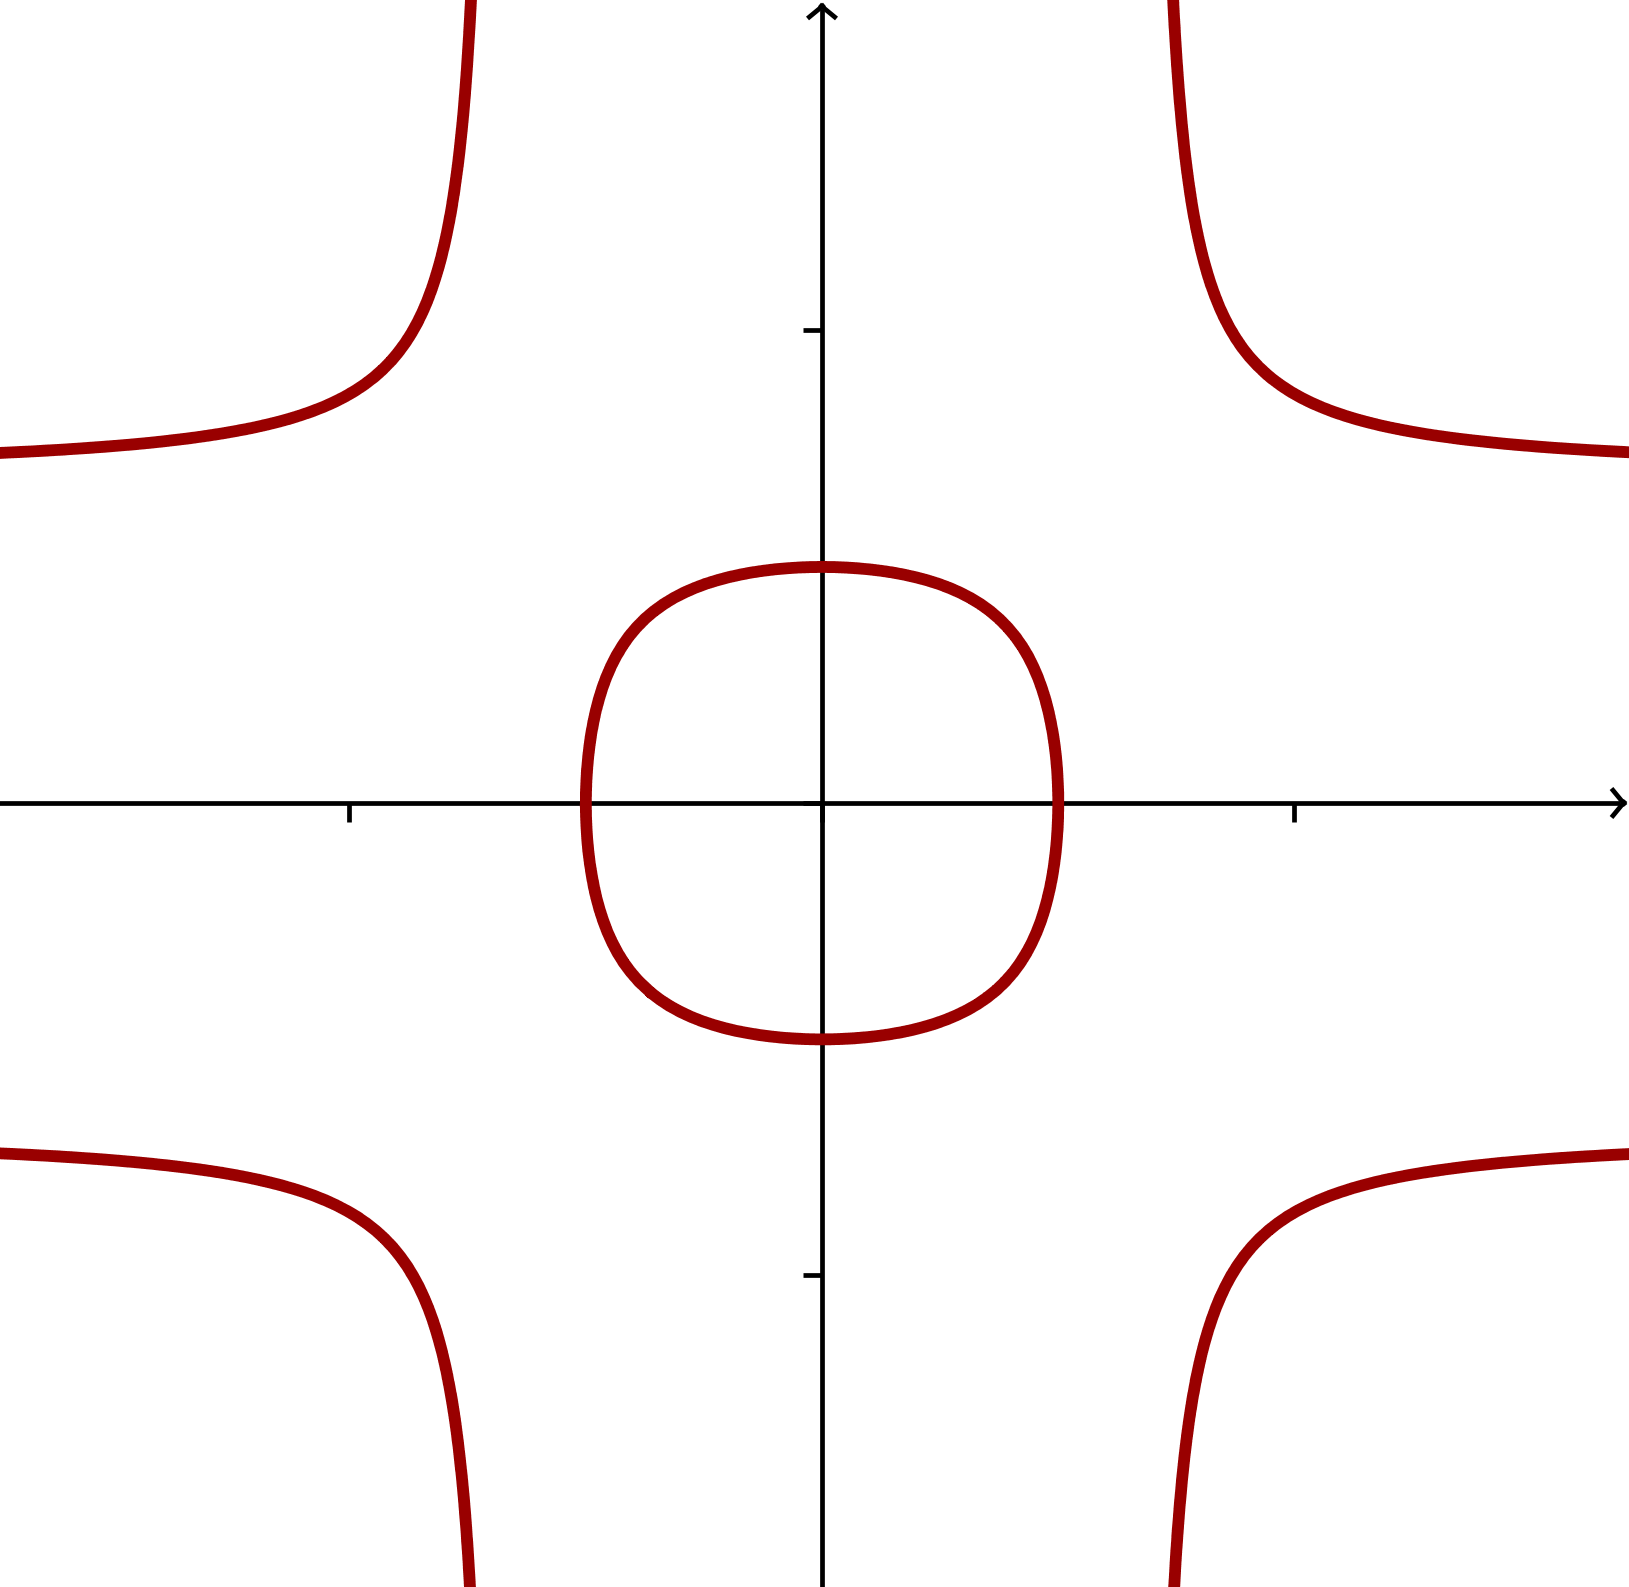
\includegraphics[scale=0.5]{edwards_curve_positive_proper.png}
\caption{Edwards curve $E_{E,\frac{1}{2}}$ over $\R$.}
\end{minipage}
\hspace{0.5cm}
\begin{minipage}[b]{0.5\linewidth}
\centering
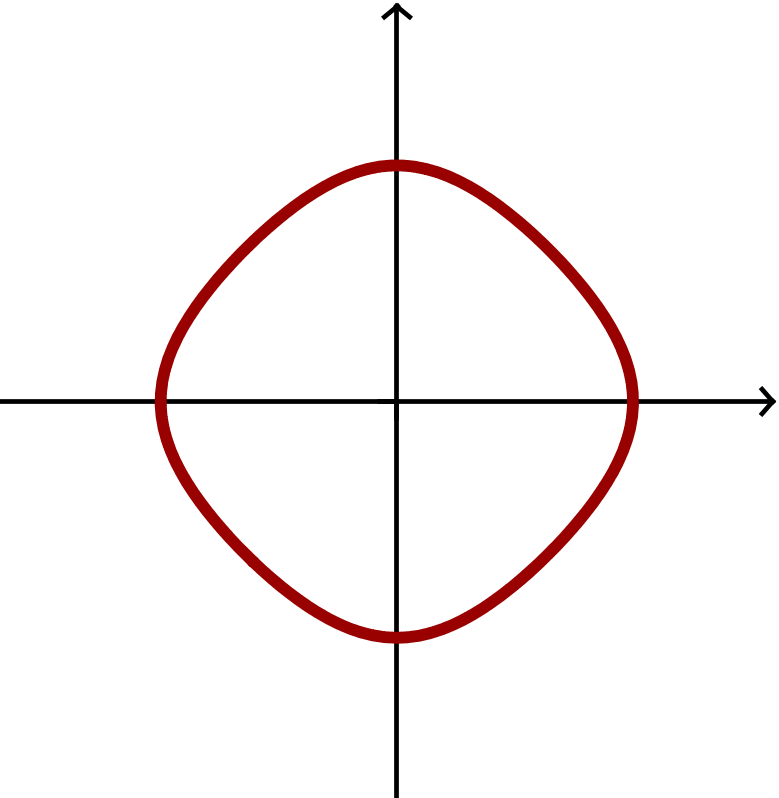
\includegraphics[scale=1]{edwards_curve_minus_one.png}
\caption{Edwards curve $E_{E,-1}$ over $\R$.}
\end{minipage}
\end{figure}
In this thesis we are interested in using Edwards curves in connection with ECM. To do this properly we must know several things: We need a lot of elliptic curves that can be written in Edwards form over the original field, addition must in some sense correspond to addition on the original elliptic curve and arithmetic on Edwards cannot be too bad otherwise it would be productive to switch to Edwards form (when one wants to be faster).

We need the notion of birationally equivalent curves. 
\begin{defn}\label{def:biratEqui}
Let $V$ and $V'$ be two curves. $V$ and $V'$ are \textit{birationally equivalent} if there exists two rational maps $\phi\,:\, V\rightarrow V'$ and $\phi'\,:\, V'\rightarrow V$ such that $\phi\circ\phi'=\text{id}$ and $\phi'\circ\phi=\text{id}$ for all but finitely many points.  
\end{defn}
First we need a connection between Edwards curves and Weierstrass curves. In the original article \cite{BL07} Bernstein and Lange used a possible twist and an assumption of existence of an unique point of order 2 on the elliptic curve, but these are redundant. The proof is completely constructive. 
\begin{thm}\label{thm:biratinal}
Let $E$ be an elliptic curve over $\F$. Assume the group $E(\F)$ has an element of order 4. Then $E$ is birationally equivalent to an Edwards curve.  
\end{thm}
\begin{proof}
Assume $E$ has a point of order 4. Let this point be $P=(l,r)$ and $r\neq 0$ otherwise $P$ would have order 2. Since $\Char(\F)\neq 2$ we may assume $E$ is on the form $v^2=u^3+a_2u^2+a_4u+a_6$. Since $P$ has order 4, $[2P]=(l',r')$ must have order 2 implying $(l',r')=(l',-r')$ and so $r'=0$. We now move this point to origo. Hence WLOG we assume $l'=0$ i.e. $[2]P=(0,0)$ and $a_6=0$; in the general case make the transformation $\overline{l}'+l'=u$. If $l=0$ we would have $r^2=0^3+a_20^2+a_40=0$ contradicting $r\neq 0$ hence $l\neq 0$.

We now express $a_2$ and $a_4$ in terms of $l$ and $r$. By the doubling law on $E$ (identity 1.8) and $[2]P=(0,0)$ we get 
\begin{align*}
	0 &= \left(\frac{3l^2+2a_2l+a_4}{2r}\right)\left(l-0\right)-r \Leftrightarrow 2r^2=3l^3+2a_2l^2+a_4l.
\end{align*}
Since $P$ is also on the curve $E$ we have the identity $r^2=l^3+a_2l^2+a_4l$. Subtracting this identity two times from the above yield
\[
	0 = l^3-a_4l \Leftrightarrow l^2=a_4
\]
because $l\neq 0$. We also obtain
\begin{align*}
	a_2 = \frac{a_2l^2}{l^2} = \frac{r^2-l^3-a_4l}{l^2} = \frac{r^2-2l^3}{l^2} = \frac{r^2}{l^2}-2l
\end{align*}
Our curve $E$ is therefore 
\begin{align}\label{identity:curve}
v^2=u^3+\left(\frac{r^2}{l^2}-2l\right)u^2+l^2u.
\end{align} 

Define $d=1-4\frac{l^3}{r^2}$. We argue $d\neq 0,1$. If $d=1$ then $l^3=0$ contradicting $l\neq 0$. If $d=0$ then $4l^3=r^2$. $E$ then has the form
\begin{align*}
	v^2 &= u^3+\left(\frac{r^2}{l^2}-2l\right)u^2+l^2u \\
		&= u^3+\left(\frac{4l^3}{l^2}-2l\right)u^2+l^2u \\
		&= u^3+2lu^2+l^2u \\
		&= u(u^2+2lu+l^2) \\
		&= u(u+l)^2
\end{align*}
implying $E$ to be a singular curve, contradicting $E$ being an elliptic curve. 

We now define a map from $E$ to the Edwards curve $E_{E,d}$ by $\varphi\, :\, (u,v)\mapsto \left(\frac{ru}{lv},\frac{u-l}{u+l}\right)$. We show this actually maps a point on $E$ to $E_{E,d}$. Put $x=\frac{ru}{lv}$ and $y=\frac{u-l}{u+l}$ then we need to show $x^2+y^2=1+dx^2y^2$. We calculate
\begin{align*}
 x^2+y^2-1-dx^2y^2 &= \frac{r^2u^2}{l^2v^2}+\frac{(u-l)^2}{(u+l)^2}-1-\left(1-4\frac{l^3}{r^2}\right)\frac{r^2u^2}{l^2v^2}\frac{(u-l)^2}{(u+l)^2} \\
 &= \frac{r^2u^2(u+l)^2+l^2v^2(u-1)^2-l^2v^2(u+l)^2-r^2u^2(u-l)^2+4l^3u^2(u-l)^2}{l^2v^2(u+l)^2}.
\end{align*}
Observe 
\begin{align*}
r^2u^2(u+l)^2-r^2u^2(u-l)^2 &= 4lr^2u^3\\
l^2v^2(u-l)^2-l^2v^2(u+l)^2 &= -4uv^2l^3.
\end{align*}
This yield
\begin{align*}
x^2+y^2-1-dx^2y^2 &= \frac{4l^3u^2(u-l)^2+4lr^2u^3-4uv^2l^3}{l^2v^2(u+l)^2} \\
&= \frac{4l^2u^2(u-l)^2+4r^2u^3-4uv^2l^2}{lv^2(u+l)^2} \\
&= \frac{4l^2u^4+4l^4u^2-8l^3u^3+4r^2u^3-4uv^2l^2}{lv^2(u+l)^2}\\
&= \frac{4u(l^2u^3+l^4u-2l^3u^2+r^2u^2-v^2l^2)}{lv^2(u+l)^2}.
\end{align*}
Since $(u,v)$ is on the curve $E$ the point satisfy identity \ref{identity:curve}. After multiplying with $l^2$ and rearranging we obtain $-l^2v^2+l^2u^3-2l^3u^2+l^4u=-r^2u^2$. Using this in the above calculation we get
\begin{align*}
	x^2+y^2-1-dx^2y^2 &= \frac{4u(r^2u^2-r^2u^2)}{lv^2(u+l)^2} = 0.
\end{align*}
Proving $x^2+y^2=1+dx^2y^2$. Exceptional points for $\varphi$ occur when $lv=0$ or $u=-l$ which clearly is only possible for finitely many points. Define a map $\psi$ from $E_{E,d}$ to $E$ by $\psi\, :\, (x,y)\mapsto \left(l\frac{1+y}{1-y},r\frac{1+y}{x(1-y)}\right)$. Script 1 in appendix A verify that $\psi$ really map from $E_{E,d}$ to $E$. The cases $y=1$ and $x=0$ are the exceptional cases and clearly occur for only finitely many points. Now
\begin{align*}
\varphi\circ\psi((u,v))&=\left(\frac{2lu(u+l)}{2l(u+l)},\frac{2lrvu(u+l)}{2lru(u+l)}\right)=(u,v) \\
\psi\circ\varphi((x,y))&=\left(\frac{rl(1+y)(1-y)x}{rl(1+y)(1-y)},\frac{2yl(1-y)}{2l(1-y)}\right)=(x,y)
\end{align*}
i.e. $\varphi \circ \psi=\text{id}$ and $\psi\circ\varphi=\text{id}$. Hence $E$ and $E_{E,d}$ are birationally equivalent. 
\end{proof}
Let $E$ be an elliptic curve over a field $\F_p$. $E$ is finite and by theorem \ref{thm:ellipticGroupComposition} also abelian. By the fundamental theorem for finite abelian groups we may write $E$ as a product of $\Z/p^k\Z$ for some primes $p$. Since any elliptic curve over a field $\F_p$ is either cyclic or a product of two cyclic groups (see \cite{pomeranceEt.al} p. 322 theorem 7.1.3) we do not have the possibility that e.g. $E=\Z/2\Z\times\Z/2\Z\times\Z/2\Z$ hence when an elliptic curve $E$ is divisible by 8 it has a point of order 4 and theorem \ref{thm:biratinal} show that $E$ is birationally equivalent to an Edwards curve. This might indicate that we have plenty of Edwards curves. 

\section{Addition on Edwards curves}\label{sec:addEdward}
We start by defining the addition law on Edwards curves.
\begin{defn}\label{def:EdwardsAddition}
Let $E_{E,d}$ be an Edwards curve and $(x_1,y_1)$, $(x_2,y_2)$ two points on it. The Edwards addition law is given by
\begin{align}\label{rel:additionsLawEdward}
	(x_1,y_1),(x_2,y_2)\mapsto \left(\frac{x_1y_2+y_1x_2}{1+dx_1x_2y_1y_2},\frac{y_1y_2-x_1x_2}{1-dx_1x_2y_1y_2}\right)
\end{align}
Addition on Edwards curves will be denoted $+$. Noting the danger of ambiguous notation, the author trusts the reader in telling from the context whether we are adding on an Edwards curve or a Weierstrass curve. 
\end{defn}

\begin{ex}\label{ex:clockGroup}
One motivation for the formula (\ref{rel:additionsLawEdward}) may be giving in the shape of the \textit{clock group}. Consider the set $\mathcal{U}$ of all tuples $(x,y)\in \F^2$ that satisfy $x^2+y^2=1$. On this set define the addition (see figure \ref{fig:clockAddition})
\[
	(x_1,y_1),(x_2,y_2)\mapsto (x_1y_2+x_2y_1,x_1x_2-y_1y_2)
\]
One may prove that this addition define a commutative composition making $\mathcal{U}$ into a group with neutral element $(0,1)$ and with each point $(x,y)$ having inverse $(-x,y)$. For $\F=\R$ we may for any point $(x,y)$ in $\mathcal{U}$ draw a straight line from that point to the origin forming an angle $\alpha$ between the positive $y$-axis and the line in the clockwise direction, see figure \ref{fig:clockAngle}. Therefore $(x,y)=(\sin\alpha,\cos\alpha)$ which can be done for all points in $\mathcal{U}$. Recall the addition laws for sine and cosine
\begin{align*}	\sin(\alpha_1+\alpha_2)=\sin\alpha_1\cos\alpha_2+\cos\alpha_1\sin\alpha_2\\	\cos(\alpha_1+\alpha_2)=\cos\alpha_1\cos\alpha_2-\sin\alpha_1\sin\alpha_2.
\end{align*}
Comparing this addition with the addition in $\mathcal{U}$ and addition on Edwards curves reveals some similarities.  
\begin{figure}[htp]
\begin{minipage}[b]{0.5\linewidth}
\centering
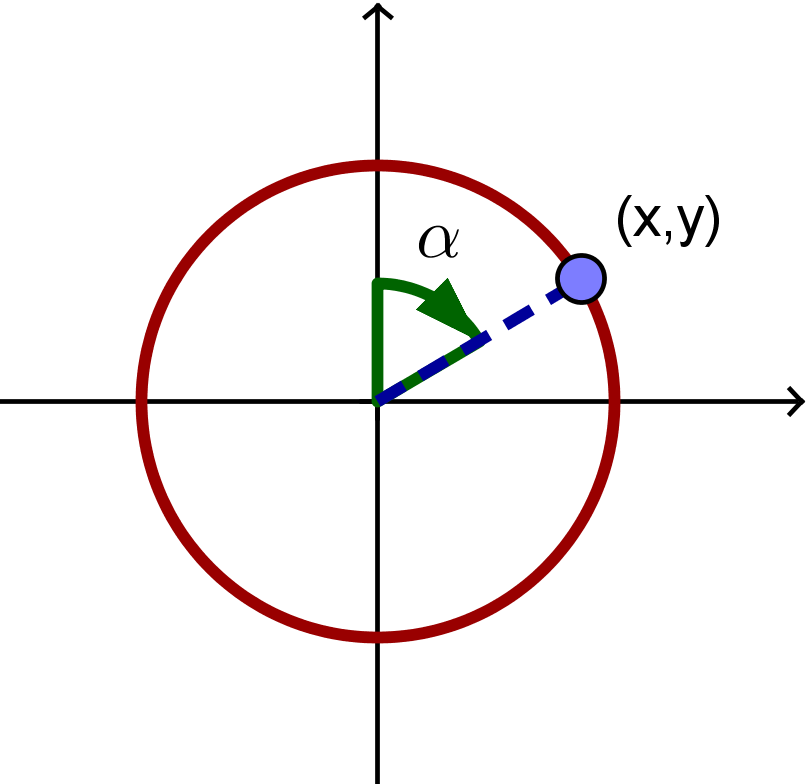
\includegraphics[scale=1]{clock_angle.png}
\caption{Angle of a point in the clock group over $\R$.}
\label{fig:clockAngle}
\end{minipage}
\hspace{0.5cm}
\begin{minipage}[b]{0.5\linewidth}
\centering
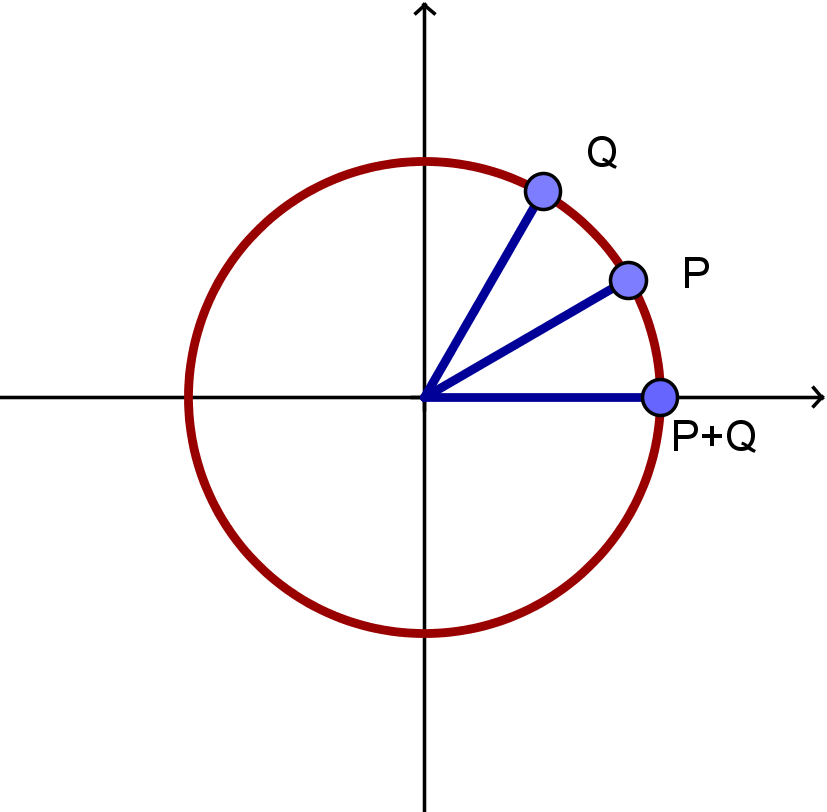
\includegraphics[scale=1]{clock_addition.png}
\caption{Addition in the clock group over $\R$. $P=\left(\frac{\sqrt{3}}{2},\frac{1}{2}\right)$, $Q=\left(\frac{1}{2},\frac{\sqrt{3}}{2}\right)$ and $P+Q=(1,0)$.}
\label{fig:clockAddition}
\end{minipage}
\end{figure}
\end{ex}
We will show that the addition law (\ref{rel:additionsLawEdward}) satisfy what we need. In theorem \ref{thm:mapsToEd} we prove that the Edwards addition maps (when defined) to the Edwards curve, theorem \ref{thm:EdCcorrespondEC} shows that ordinary addition on the birationally equivalent elliptic curve in \ref{thm:biratinal} corresponds to addition on the Edwards curve. Finally in theorem \ref{thm:complete} we prove a very strong property Edwards addition possess. 
\begin{rem}
The neutral element for Edwards addition is $(0,1)$ and the inverse for a point $(x,y)$ is $(-x,y)$. An Edwards curve always has two points of order 4 namely $(1,0)$ and $(-1,0)$. This is immediate from the calculation
\begin{align*}
&(1,0)+(1,0)+(1,0)+(1,0)=(0,-1)+(0,-1)=(0,1) \\
&(-1,0)+(-1,0)+(-1,0)+(-1,0)=(0,-1)+(0,-1)=(0,1)
\end{align*}
Notice that $\{(0,1),(0,-1),(1,0),(-1,0)\}$ defines a group with the Edwards addition. In general the addition formula is unified; it works for both squaring and addition. 
\end{rem}
\begin{thm}\label{thm:mapsToEd}
Let $E_{E,d}$ be an Edwards curve and let $(x_1,y_1),(x_2,y_2)$ be points on $E_{E,d}$. Assume $1\pm dx_1x_2y_1y_2\neq 0$. Define $x_3=\frac{x_1y_2+y_1x_2}{1+dx_1x_2y_1y_2}$ and $y_3=\frac{y_1y_2-x_1x_2}{1-dx_1x_2y_1y_2}$. Then $(x_3,y_3)$ is a point on $E_{E,d}$. 
\end{thm}
\begin{proof}
There is really no magic involved in this proof - only humdrum. We must prove $x_3^2+y_3^2=1+dx_3^2y_3^2$. 

First we need an identity. Let
\begin{align*}
	\delta = (x_1y_2+y_1x_2)^2(1-dx_1x_2y_1y_2)^2+(y_1y_2-x_1x_2)^2(1+dx_1x_2y_1y_2)^2
\end{align*} 
Then one can check with e.g. Sage or Maple, the following
\begin{align*}
	\delta = (x_1^2+y_1^2-(x_2^2+y_2^2)dx_1^2y_1^2)(x_2^2+y_2^2-(x_1^2+y_1^2)dx_2^2y_2^2)+d(x_1y_2+y_1x_2)^2(y_1y_2-x_1x_2)^2
\end{align*}
Script 2 in appendix A verifies this. Since $(x_1,y_1)$ and $(x_2,y_2)$ are both points on $E_{E,d}$ they satisfy
\begin{align}
 x_1^2+y_1^2&=1+dx_1^2y_1^2\label{id:1} \\
 x_2^2+y_2^2&=1+dx_2^2y_2^2\label{id:2}.
\end{align}
Multiplying (\ref{id:1}) with $dx_2^2y_2^2$ and subtracting the new identity from (\ref{id:2}) yield
\begin{align}\label{id:3}
	x_2^2+y_2^2-(x_1^2+y_1^2)dx_2^2y_2^2 = 1-(dx_1x_2y_1y_2)^2.
\end{align}
Similarly by multiplying (\ref{id:2}) with $dx_1^2y_1^2$ and subtraction this from (\ref{id:1}) we get
\begin{align}\label{id:4}
	x_1^2+y_1^2-(x_2^2+y_2^2)dx_1^2y_1^2 = 1-(dx_1x_2y_1y_2)^2.
\end{align}
When substituting (\ref{id:3}) and (\ref{id:4}) into the identity for $\delta$ we obtain
\begin{align*}
\delta = (1-(dx_1x_2y_1y_2)^2)^2+d(x_1y_2+y_1x_2)^2(y_1y_2-x_1x_2)^2.
\end{align*}
The finishing touch is obvious now:
\begin{align*}
	x_3^2+y_3^2 &=  \left(\frac{x_1y_2+y_1x_2}{1+dx_1x_2y_1y_2}\right)^2+\left(\frac{y_1y_2-x_1x_2}{1-dx_1x_2y_1y_2}\right)^2 \\
	&= \frac{(x_1y_2+y_1x_2)^2(1-dx_1x_2y_1y_2)^2+(y_1y_2-x_1x_2)^2(1+dx_1x_2y_1y_2)^2}{(1+dx_1x_2y_1y_2)^2(1-dx_1x_2y_1y_2)^2} \\
	&= \frac{\delta}{(1+dx_1x_2y_1y_2)^2(1-dx_1x_2y_1y_2)^2} \\
	&= \frac{(1-(dx_1x_2y_1y_2)^2)^2+d(x_1y_2+y_1x_2)^2(y_1y_2-x_1x_2)^2}{(1+dx_1x_2y_1y_2)^2(1-dx_1x_2y_1y_2)^2} \\
	&= \frac{(1-(dx_1x_2y_1y_2)^2)^2}{(1-(dx_1x_2y_1y_2)^2)^2}+d\frac{(x_1y_2+y_1x_2)^2(y_1y_2-x_1x_2)^2}{(1+dx_1x_2y_1y_2)^2(1-dx_1x_2y_1y_2)^2} \\
	&=1+d\left(\frac{x_1y_2+y_1x_2}{1+dx_1x_2y_1y_2}\right)^2\left(\frac{y_1y_2-x_1x_2}{1-dx_1x_2y_1y_2}\right)^2 \\
	&= 1+dx_3^2y_3^2.
\end{align*}
\end{proof}
Script 3 in appendix A also verifies theorem \ref{thm:mapsToEd}. Imagine an application where you need to calculate a series of computations on an elliptic curve say $nP_1+mP_2$ were $P_1$ and $P_2$ are points on the curve. If $n$ and $m$ are large, reducing the cost of addition on the elliptic curve is preferable. In section \ref{sec:effAddandAna} we will see that arithmetic on Edwards curves are way faster than arithmetic on a Weierstrass curve. Actually we will see that arithmetic on Edwards curves is superior to almost all known schemes of addition on elliptic curves. 

The following shows that it is possible to change to an Edwards curve if there exists a biratinal equivalence between an Edwards curve and the elliptic curve. 
\begin{thm}\label{thm:EdCcorrespondEC}
Assume the situation from theorem \ref{thm:mapsToEd}. Let $E_{E,d}$ be an Edwards curve and $E$ be the elliptic curve $\frac{1}{1-d}v^2=u^3+2\left(\frac{1+d}{1-d}\right)u^2+u$. For $i=1,2,3$ define
\begin{align}\label{assignments}
P_i = \begin{cases}
	\infi & (x_i,y_i)=(0,1) \\
	(0,0) & (x_i,y_i)=(0,-1) \\
	\left(\frac{1+y_i}{1-y_i},2\frac{1+y_i}{(1-y_i)x_i}\right) & x_i\neq 0
\end{cases}
\end{align}
where $(x_i,y_i)$ are points on $E_{E,d}$ and $(x_1,y_1)+(x_2,y_2)=(x_3,y_2)$. Then $P_i\in E(\F)$ and $P_1+P_2=P_3$. 
\end{thm} 
\begin{proof}
Notice that if $y_i=1$ then $x^2+1=1+dx^2$ if and only if $x^2(1-d)=0$. Hence $x=0$ otherwise $d=1$ contradicting $E_d$ being an Edwards curve. That is, in (\ref{assignments}) we will not assign $P_i$ with the last case when $y_i=1$.

We show $P_i\in E(\F)$ by splitting into the three cases in (\ref{assignments}). The first two are obvious. Therefore assume the last case. Put $x_i=x$ and $y_i=y$. We simple calculate
\begin{align*}
&\frac{(1-y)^3(1-d)}{y+1}\left(\left(\frac{1+y}{1-y}\right)^3+2\left(\frac{1+d}{1-d}\right)\left(\frac{1+y}{1-y}\right)^2+\frac{1+y}{1-y}\right) \\
&=(1+y)^2(1-d)+2(1+d)(1+y)(1-y)+(1-y)^2(1-d) \\
&=(1+2y+y^2)(1-d)+2(1+d)(1-y^2)+(1-2y+y^2)(1-d) \\
&=1+2y+y^2-d-2dy-dy^2+2-2y^2+2d-2dy^2+1-2y+y^2-d+2dy-dy^2 \\
&=4(1-dy^2)\\
&=4\left(1-\frac{1-x^2-y^2}{x^2}\right) \\
&=4\frac{(1-y)(1+y)}{x^2}.
\end{align*}
Multiply through with $\frac{y+1}{(1-y)^3(1-d)}$ to obtain
\[
\left(\frac{1+y}{1-y}\right)^3+2\left(\frac{1+d}{1-d}\right)\left(\frac{1+y}{1-y}\right)^2+\frac{1+y}{1-y} = 
4\frac{(1+y)^2}{(1-y)^2x^2}=\left(2\frac{1+y}{(1-y)x}\right)^2
\]
Proving $P_i\in E(\F)$. 

We are left with the task of proving $P_1+P_2=P_3$. This will split into several cases. 

If $(x_1,y_1)=(0,1)$ then $P_1=\infi$ and $(x_3,y_3)=(x_1,y_1)+(x_2,y_2)=(x_2,y_2)$. Thus $P_1+P_2=\infi+P_2=P_2=P_3$. Same arguments work if $(x_2,y_2)=(0,1)$. For the rest we therefore assume $(x_1,y_1)$ and $(x_2,y_2)$ is not $(0,1)$. 

If $(x_3,y_3)=(0,1)$ then $(x_1,y_1)=(-x_2,y_2)$ and $P_3=\infi$. We must show $P_1=-P_2$. Suppose $(x_1,y_1)=(0,-1)$ then $(x_2,y_2)=(0,-1)$ and $P_1=(0,0)=P_2$ so $P_1=-P_2$. Symmetric if $(x_2,y_2)=(0,-1)$. If the latter is not the case, $x_1,x_2\neq 0$. Then
\begin{align*}
	P_1=\left(\frac{1+y_1}{1-y_1},2\frac{1+y_1}{(1-y_1)x_1}\right)=\left(\frac{1+y_2}{1-y_2},2\frac{1+y_2}{(1-y_2)(-x_2)}\right)=-P_2
\end{align*}  
From now on assume $(x_3,y_3)\neq (0,1)$

If $(x_1,y_1)=(0,-1)$ then $P_1=(0,0)$ and $(x_3,y_3)=(0,-1)+(x_2,y_2)=\left(\frac{-x_2}{1},\frac{-y_2}{1}\right)=(-x_2,-y_2)$. This imply $(x_2,y_2)\neq (0,-1)$ otherwise $(x_3,y_3)=(0,1)$ which has been handled. Thus $x_2\neq 0$ and we have 
\[
	u_2=\frac{1+y_2}{1-y_2},\quad v_2=2\frac{1+y_2}{(1-y_2)x_2}=2\frac{u_2}{x_2}
\]
such that $P_2=(u_2,v_2)$. $u_2$ and $v_2$ satisfy $\frac{1}{1-d}v_2^2 = u_2^3+2\frac{1+d}{1-d}u_2^2+u_2$ (by theorem \ref{thm:mapsToEd}). Multiplying with $\frac{1}{u_2^2}$ ($y_2\neq -1$ hence $u_2\neq 0$) and rearranging we get $\frac{1}{1-d}\left(\frac{v_2}{u_2}\right)^2-u_2-2\frac{1+d}{1-d}=\frac{1}{u_2}$. Now standard addition on $E$ give $P_1+P_2=(0,0)+(u_2,v_2)=(l_3,r_3)$ where
\begin{align*}
	l_3 &= \frac{1}{1-d}\left(\frac{v_2-0}{u_2-0}\right)^2-2\frac{1+d}{1-d}-u_2-0 = \frac{1}{u_2} \\
	r_3 &= \frac{v_2-0}{u_2-0}\left( 0-l_3\right)-0 =-\frac{v_2}{u_2^2} 
\end{align*}
Also
\begin{align*}
	P_3 &= \left(\frac{1+y_3}{1-y_3},2\frac{1+y_3}{(1-y_3)x_3}\right)
	    = \left(\frac{1-y_2}{1+y_2},-2\frac{1-y_2}{(1+y_2)x_2}\right)
	    = \left(\frac{1}{u_2},-2\frac{1}{u_2x_2}\right)\\
	    &= \left(l_3,-2\frac{u_2}{u_2^2x_2}\right)
		= \left(l_3,-\frac{v_2}{u_2^2}\right)
		= \left(l_3,r_3\right)
\end{align*}
Thus $P_1+P_2=P_3$. If $(x_2,y_2)=(0,-1)$ similar arguments apply. 

For the rest of this proof we assume $x_1,x_2\neq 0$. We can now put $P_i=(u_i,v_i)$ with $u_i=\frac{1+y_i}{1-y_i}$ and $v_i=2\frac{u_i}{x_i}$ for $i=1,2$. 

If $(x_3,y_3)=(0,-1)$ then $(x_1,y_1)=(x_1,y_1)+(x_2,y_2)-(x_2,y_2)=(x_3,y_3)-(x_2,y_2)=(0,-1)+(-x_2,y_2)=(x_2,-y_2)$ and $P_3=(0,0)$. With almost the same calculations as before $u_1=\frac{1}{u_2}$ and $v_1=\frac{v_2}{u_2^2}$. As before we have
\[
	-P_3+P_2=(0,0)+P_2=\left(\frac{1}{u_2},-\frac{v_2}{u_2^2}\right)=(u_1,-v_1)=P_1
\]
proving $P_1+P_2=P_3$. Script 4 in appendix A verifies that $P_1+P_2=P_3$ in the above case. Now we can also assume $x_3\neq 0$ and put $P_3=(u_3,v_3)$ with $u_3=\frac{1+y_3}{1-y_3}$ and $v_3=2\frac{u_3}{x_3}$. 

If $P_1=-P_2$ then $u_1=u_2$ and $v_1=-v_2$. Thus $x_1=2\frac{u_1}{v_1}=2\frac{u_2}{v_2}=x_2$ and $y_1=\frac{u_1-1}{u_1+1}=\frac{u_2-1}{u_2+1}=-y_2$ implying $(x_3,y_3)=(0,1)$. This case has already been handled. Assume form now on that $P_1\neq -P_2$. 

If $u_1=u_2$ and $v_1\neq -v_2$ (we assume $P_1\neq -P_2$). Then by the standard addition law we get $l_3=\frac{1}{1-d}m^2-2\frac{1+d}{1-d}-2u_1$, $r_3=m(u_1-l_3)-v_1$, $m=\frac{3u_1^2+4((1+d)/(1-d))u_1+1}{(2/(1-d))v_1}$ where $(x_1,y_1)+(x_2,y_2)=(l_3,r_3)$. As before it is (with a lot of paper) straight forward to verify $(l_3,r_3)=(u_3,v_3)$.

Last(!) case: If $u_1\neq u_2$. Again using the standard addition law we obtain $m=\frac{v_2-v_1}{u_2-u_1}$, $l_3=\frac{1}{1-d}m^2-2\frac{1+d}{1-d}-u_1-u_2$ and $r_3=m(u_1-l_3)-v_1$ with $(u_1,v_1)+(u_2,v_2)=(l_3,r_3)$. One can again check that $(l_3,r_3)=(u_3,v_3)$. This and the latter case is checked in \cite{EFD}.

We are done!
\end{proof}
\begin{rem}
\label{rem:commentsProof}
In the proof above we used several times that the only points on an Edwards curve with zero $x$-coordinate are $(0,1)$ and $(0,-1)$. This is immediate if we substitute $x=0$ in the defining equation of an Edwards curve: $1=y^2$ so $0=(1-y)(1+y)$. We also used a generalized form of addition; an elliptic curve on the form $By^2 = x^3+cx^2+x$ is called a Montgomery curve. Addition formulas for this kind of curve differ a little with respect to the usual addition formulas for addition on elliptic curves. Namely (\ref{add1}) change to $x_3=Bm^2-c-x_1-x_2$, (\ref{add2}) stays as it is and 
\begin{align*}
	m = \begin{cases} 
		\frac{y_2-y_1}{x_2-y_2} & x_2\neq x_1 \\
		\frac{3x_1^2+2cx_1+a}{2By_1} & x_2= x_1
		\end{cases}				
\end{align*}
\end{rem}
 
We can now show that the condition in theorem \ref{thm:biratinal} is not only a sufficient condition but a necessary condition. 
\begin{thm}\label{thm:pointoforderfour}
Let $E$ be an elliptic curve over $\F$. If $E$ is birationally equivalent to an Edwards curve, the group $E(\F)$ has an element of order 4. 
\end{thm}
\begin{proof}
Assume $E$ is birationally equivalent over $\F$ to an Edwards curve $E_{E,d}$. With the rational map $(x,y)\mapsto \left(\frac{1+y}{1-y},2\frac{1+y}{(1-y)x}\right)$ we map points on $E_{E,d}$ too the elliptic curve $E':\quad\frac{1}{1-d}v^2=u^3+2\frac{1+d}{1-d}u^2+u$. The inverse map is $(u,v)\mapsto \left(2\frac{u}{v},\frac{u-1}{u+1}\right)$. This gives a birationally equivalence between $E_{E,d}$ and $E'$ thus also a birationally equivalence between $E$ and $E'$. In theorem \ref{thm:EdCcorrespondEC} we saw that addition on $E_{E,d}$ corresponds to addition on the elliptic curve $E'$. Since the point $(1,0)$ on $E_{E,d}$ has order 4 the corresponding point on $E'$ also has order 4 and $E$ must have a point of order 4.  
\end{proof}

It turns out that in some cases the addition formula on Edwards curves is even complete i.e works for all input; in this case any addition on the Edwards is without risk of failure. 
\begin{thm}\label{thm:complete}
Let $E_{E,d}$ be an Edwards curve. Assume $d$ is \textit{not} a square. Let $(x_1,y_1)$ and $(x_2,y_2)$ be points on $E_{E,d}$. Then $1\pm dx_1x_2y_1y_2\neq 0$. 
\end{thm} 
\begin{proof}
This will be a proof by contradiction. Let $\delta = dx_1x_2y_1y_2$ and suppose for the sake of contradiction that $\delta=\pm 1$. It follows $x_1,x_2,y_1,y_2\neq 0$. Then 
\begin{align*}
(x_1+\delta y_1)^2 &= x_1^2 +\delta^2 y_1^2+2x_1y_1\delta
= x_1^2 + (-1)^2y_1^2+2x_1y_1\delta \\
&= 1+dx_1^2y_1^2+2x_1y_1\delta 
= \delta^2 +dx_1^2y_1^2+2x_1y_1\delta \\
&= dx_1^2y_1^2+d^2x_1^2x_2^2y_1^2y_2^2+2x_1y_1\delta 
= dx_1^2y_1^2(1+dx_2^2y_2^2)+2x_1y_1\delta \\
&= dx_1^2y_1^2(x_2^2+y_2^2)+2x_1y_1\delta
= dx_1^2y_1^2(x_2^2+y_2^2)+2x_1y_1d^2x_1^2x_2^2y_1^2y_2^2 \\
&= dx_1^2y_1^2(x_2^2+2x_2y_2+y_2^2) 
= dx_1^2y_1^2(x_2+y_2)^2.
\end{align*}
If $x_2+y_2\neq 0$ (recall $x_1,y_1\neq 0$) then $d=\left(\frac{x_1+\delta y_1}{x_1y_1(x_2+y_2)}\right)^2$ contradicting $d$ being a non-square. One can do similar calculations as above and get $(x_1-\delta y_1)^2=dx_1^2y_1^2(x_2-y_2)^2$. If $x_2-y_2\neq 0$ then $d=\left(\frac{x_1-\delta y_1}{x_1y_1(x_2-y_2)}\right)^2$ contradiction. Hence $x_2+y_2=0$ and $x_2-y_2=0$. We quickly spot $0=(x_2+y_2)+(x_2-y_2)=2x_2$ and $0=2y_2$. Since $\Char(\F)\neq 2$ we get $x_2,y_2=0$ our final contradiction. 
\end{proof}

We will be using this property in the implementation since we go for speed not for this simplicity or as we shall see now, security. Consider an implementation of some cryptographic scheme using double-scaler-multiplication on elliptic curves i.e $[n]P+[m]Q$. The usual addition formulas for the Weierstrass model has several exceptional cases and an irritating distinction between addition and doubling; you can not double a point as $P+P$ and use the addition formula. The plethora of cases has caused a variety of problems, in particular, when in \cite{Kocher96timingattacks} Paul Kocher described a timing attack of several widely used crypto systems an laid the ground for side-channel attacks. In recent times timing attacks are exploiting the property that addition and doubling are different operations enabling that the involved secrets could be revealed from only a single execution of the used algorithm. Several countermeasures such as adding dummy operations or rewriting formulas are known and used, but the complete addition formula for Edwards curves solves this in one sweep move.

\section{Efficient operations on Edwards curves}\label{sec:effAddandAna}
In this section we introduce efficient formulas for computing on Edwards curves and compare these formulas to other popular schemes. Efficiency of the operations are ordered by the number of operations in the underlying field. In particular we count; number of multiplications \textbf{M} (each costing \textbf{M}), number of squarings \textbf{S} (each costing \textbf{S}), multiplication by $d$ costing \textbf{D} (each costing \textbf{D}) and number of additions/subtractions \textbf{A} (each costing \textbf{A}). We do not keep track of inversions since we avoid these by using projective coordinates. 

The reader may wonder why we keep a separate tally of squaring when a squaring is essentially a multiplication. It is true that squaring and multiplication both has the same complexity, but multiplication algorithms normally simplify when inputting a square which will speed up squaring by a constant factor. 

The reason for avoiding inversions is the known fact that inversions is inefficient compared to doing multiplications or additions. Of course the ratio inversion/multiplication differ depending on which platform and hardware being used, but generally one should expect a factor that is quite high. For instance in \cite{EFD} Bernstein and Lange use $I/M=100$.

To avoid inversions when computing on Edwards curves we homogenize the Edwards curve to $(x^2+y^2)z^2=z^4+dx^2y^2$. A point $[x,y,z]$ corresponds to the affine point $\left(\frac{x}{z},\frac{y}{z}\right)$ for $z\neq 0$. Putting the two points $\left(\frac{x_1}{z_1},\frac{y_1}{z_1}\right)$ and $\left(\frac{x_2}{z_2},\frac{y_2}{z_2}\right)$ into the addition formula for the Edwards curve yields
\begin{align*}
\frac{\frac{x_1y_2+x_2y_1}{z_1z_2}}{1+\frac{dx_1x_2y_1y_2}{z_1^2z_2^2}} &= \frac{(x_1y_2+x_2y_1)z_1z_2}{z_1^2z_2^2+dx_1x_2y_1y_2} =  \frac{(x_1y_2+x_2y_1)z_1z_2(z_1^2z_2^2-dx_1x_2y_1y_2)}{(z_1^2z_2^2)^2-(dx_1x_2y_1y_2)^2} \\
\frac{\frac{y_1y_2-x_1x_2}{z_1z_2}}{1-\frac{dx_1x_2y_1y_2}{z_1^2z_2^2}} &=\frac{(y_1y_2-x_1x_2)z_1z_2(z_1^2z_2^2+dx_1x_2y_1y_2)}{(z_1^2z_2^2)^2-(dx_1x_2y_1y_2)^2}.
\end{align*}
Put $\delta = dx_1x_2y_1y_2$. Addition on the projective form of the Edwards curve is (with $z_1,z_2\neq 0$)
\begin{align*}
&\left([x_1,y_1,z_1],[x_2,y_2,z_2]\right)\overset{ADD}\mapsto \\ 
&\left( (x_1y_2+x_2y_1)z_1z_2(z_1^2z_2^2-\delta),(y_1y_2-x_1x_2)z_1z_2(z_1^2z_2^2+\delta),(z_1^2z_2^2)^2-\delta^2\right).
\end{align*}
The neutral element is $[0,1,1]$ and if $[x,y,z]$ is a point on the homogenized curve then $[-x,y,z]$ is the inverse. Rewriting $x_1y_2+x_2y_1=(x_1+x_2)(y_1+y_2)-x_1x_2-y_1y_2$ and exploiting    different common sub expressions one may count 10\textbf{M}+1\textbf{S}+1\textbf{D}+7\textbf{A} for one addition.

In some cases we may save 1\textbf{M} namely in a mixed addition; an additions with $z_2=1$. In this case we do not need to do the calculation $z_1z_2$. The count for mixed addition then reads 9\textbf{M}+1\textbf{S}+1\textbf{D}+7\textbf{A} for one mixed addition.

Doublings are even faster. Using the ordinary addition on Edwards curves with two equal points yield
\begin{align*}
\left(\frac{xy+yx}{1+dx^2y^2},\frac{y^2-y^2}{1-dx^2y^2}\right)&=\left(\frac{2xy}{x^2+y^2},\frac{y^2-x^2}{2-x^2-y^2}\right) = \left( \frac{2xy}{x^2+y^2},\frac{x^2-y^2}{x^2+y^2-2}\right)
\end{align*}
using that $(x,y)$ satisfy $x^2+y^2=1+dx^2y^2$. In projective coordinates the doubling formula is ($z\neq 0$)
\begin{align*}
\left([x,y,z]\right)\overset{DUP}\mapsto \left( 2xy(2z^2-(x^2+y^2)),(x^2-y^2)(x^2+y^2),(x^2+y^2)(x^2+y^2-2z^2)\right).
\end{align*}
Again rewriting $2xy=(x+y)^2-x^2-y^2$ and exploiting common sub expressions we count 3\textbf{M}+4\textbf{S}+6\textbf{A} for one duplication. Notice this formula is independent of $d$.

Register allocations for the above formulas are given in section \ref{sec:SSM} where one easily read of the counts stated above. 

In \cite{BL07} Bernstein and Lange among other things, did a survey on the efficiency of several additions schemes in the literature. They gathered addition and squaring counts for different curves and coordinates systems and compared them. The results presented in their article clearly shows that Edwards curves provide one of the fastest addition and squaring known in the literature. Using Edwards curves Bernstein and Lange has discovered even faster formulas. In \cite{inv} they presented \textit{inverted edwards coordinates}; a point $[x,y,z]$ with $xyz\neq 0$  on the projective curve $(x^2+y^2)z^2=x^2y^2+dz^4$ corresponds to $\left(\frac{z}{x},\frac{z}{y}\right)$. They report costs of addition and squarings as: 9\textbf{M}+1\textbf{S}+1\textbf{D}+1\textbf{A} and 3\textbf{M}+4\textbf{S}+1\textbf{D}+1\textbf{A} respectively. Compared to the provious formalus we trade 1\textbf{M} in the addition formula with a 1\textbf{D} in the doubling formula. 

